%!TEX root = FreeRtos ARM uController.tex
\subsection{Low Power Modes auf Stm32F4}
\label{sec:Low Power Modes}
Echtzeitbetriebssysteme werden immer häufiger in akkubetriebenen embedded Systemen eingesetzt. Solche Systeme verlangen eine effiziente Nutzung der Energieressourcen, um einen möglichst langen Betrieb zu ge\-währ\-leis\-ten. Bezogen auf den $\mu$\-Pro\-zesso\-r gibt es zwei Wege zur Energieeinsparung:
\begin{itemize}
	\item Heruntertakten des $\mu$\-Pro\-zesso\-rs.
	\item Das System schlafen legen, wenn keine weiteren Aufgaben anstehen.
\end{itemize}
Das Heruntertakten des $\mu$\-Pro\-zesso\-rs ist unabhängig vom Einsatz eines RTOS. Aus diesem Grund wird hier nur der zweite Punkt genauer betrachtet, das Schlafenlegen des $\mu$\-Pro\-zesso\-rs. 
\begin{figure}[htb!]
	\centering
		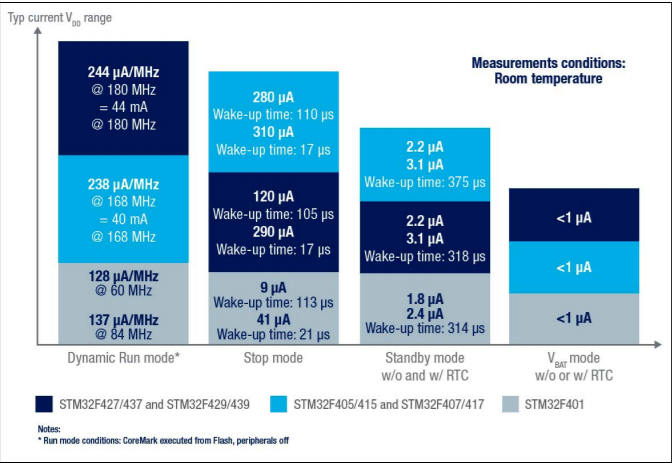
\includegraphics[width=0.4\textwidth]{Pictures/STM32F4/powerConsumption.png}
	\caption{Der STM32F4 bietet diverse LowPower Modes. Die Modes haben starke Auswirkung auf die Funktionalität des uControllers während der Schlafphase. Beispielsweise kann im Stop Mode keine UART Schnittstelle benutzt werden. Abhängig von der benötigten Peripherie, wählt der Entwickler einen dieser Modes. Die genutzte Taktfrequenz hat ebenfalls Einfluss auf die Stromaufnahme. Eine Anpassung der Takfrequenz zur Laufzeit ist ebenfalls möglich.}
	\quelle{STM32F4 - Power Modes}
	\label{fig:powerconsum}
\end{figure}
Abbildung \ref{fig:powerconsum} zeigt wie sich die Stromaufnahme beim STM32F4 von 40mA im Normalbetrieb(bei 168 MHz) auf 2,2$\mu$A im Tiefschlafmodus reduzieren lässt. 
In einfachen Anwendungen ist der Zustand, in dem ein Gerät schlafen gehen kann, relativ leicht zu ermitteln.\newline In komplexen Systemen ist die Ermittlung dieses Zustands aufwendiger, da mehrere Tasks mög\-li\-cherweise auf unterschiedliche Ressourcen warten. Ein Echtzeitbetriebssystem, wie FreeRTOS, kann hierbei unterstützen. In diesem Abschnitt wird gezeigt, welche Funktionen FreeRTOS zur Ver\-fü\-gung stellt, um einen energieeffizienten Betrieb zu ge\-währ\-leis\-ten. Eine Mög\-lich\-keit ist die Idle-Hook Funktion. Wie bereits in Abschnitt \ref{Scheduling} beschrieben, wird der IDLE Task von FreeRTOS aktiviert, sobald sich alle User-Tasks im Blocked Zustand befinden. Durch konfigurieren des Präprozessor-Defines        
\begin{lstlisting}[label=lst:defineIdleHook, numbers = none]
#define configUSE_IDLE_HOOK  1; 
\end{lstlisting}
kann die Idle-Hook Funktion aktiviert werden. Diese wird immer aufgerufen, sobald der Idle Task in den Zustand Running wechselt. Die Funktionalität der Idle-Hook Funktion kann frei vom Entwickler implementiert werden. 
\begin{lstlisting}[caption={Pseudocode für eine Idle-Hook Funktion},captionpos=b, label=lst:xIdleHookExamp, float=hbt!]
extern "C" void vApplicationIdleHook( void ){
	/* Systick Interrupt deaktivieren */
	SysTick->CTRL &= ~SysTick_CTRL_TICKINT_Msk;
	//RTC konfigurieren
	setRTCWakeupTime();
	//externen Interrupt durch RTC aktivieren
	enableRTCInterrupt();
	//deaktiviere alle anderen Interrupt Quellen
	deactivateExternalDevices();
	setAllGPIOsToAnalog(); 
	disableGPIOClocks();
	//MCU stoppen und schlafen ZzZZz
	HAL_PWR_EnterSTOPMode(PWR_LOWPOWERREGULATOR_ON, PWR_STOPENTRY_WFI); 
	//Aufgewacht...the show must go on
	//aktiviere Systick
	SysTick->CTRL |= SysTick_CTRL_TICKINT_Msk;
	//reaktiviere GPIO Clocks
	enableGPIOClocks();
	//reaktiviere Externe Interrupt Quellen
	enableExternalInterrupts();	
}
\end{lstlisting}
\newline  %Sonst zerreist es das Listing über die Abbildung
Listing \ref{lst:xIdleHookExamp} zeigt Pseudocode zu einer beispielhaften Implementierung der Idle-Hook Funktion. Bevor das System schlafen gelegt werden kann, müssen alle GPIOs und IRQs konfiguriert werden, sodass das System nicht unnötigerweise aufwacht. Des Weiteren werden alle nicht benötigten GPIOs auf Analog gestellt um Energie zu sparen. Als einzige Interrupt-Quelle wird hier eine externe RTC konfiguriert. Mit dem Aufruf von HAL\_PWR\_EnterSTOPMode() wird der $\mu$\-Pro\-zesso\-r in den Schlafmodus versetzt. Die Funktion wird erst wieder verlassen, wenn der externe Interrupt der RTC ausgelöst wurde. Danach werden alle GPIOs auf den ursprünglichen Zustand zurückgesetzt. Auserdem sind die User-Tasks zu informieren, z.B. mittels Notify oder Message, damit das System nicht beim nächsten Tick Interrupt den Idle Task reaktiviert. Nachteil dieser Variante ist, dass die Nutzung von Software Timern nicht mehr möglich ist. Der FreeRTOS Kernel würde in diesem Fall die Idle-Hook Funktion aufrufen und sich schlafen legen, obwohl noch Software Timer aktiv sind. Die Nutzung von absoluten Zeiten ist ebenfalls nicht mehr möglich, da nach der Deaktivierung des Tick Interrupts der Tickcount nicht mehr korrekt ist. Abhilfe schafft hier eine weitere Funktionalität die FreeRTOS zur Verfügung stellt, der sogenannte Tickless Idle Mode. Der Tickless Idle Mode kann durch das folgende Define in der FreeRTOSconfig.h aktiviert werden.  
\begin{lstlisting}[label=lst:defineTicklessIdle, numbers = none]
#define configUSE_TICKLESS_IDLE  1; 
\end{lstlisting}
Im Gegensatz zur gewöhnlichen Idle-Hook Funktion be\-rück\-sich\-tigt der Tickless Idle Mode alle ausstehenden Timerfunktionen, dazu gehören neben allen Software Timern auch Tasks, die nur für eine gewisse Zeit blockiert sind, z.B. durch die Funktion xTaskWaitUntil(). Des Weiteren muss der Tickinterrupt nicht, wie in Listing \ref{lst:xIdleHookExamp} dargestellt, explizit abgeschaltet werden. Dies wird hier automatisch durch den Kernel gehandelt. Der Tickless Idle Mode bietet durch die Funktion vTaskStepTick() auch die Möglichkeit den TickCount nach dem Aufwachen anzupassen. Die verpassten TickCounts können beispielsweise durch einen externen Timer oder die RTC bestimmt werden. So ist es auch möglich Software Timer für absolute Zeiten zu nutzen. Details und Beispiel Implementierungen hierzu finden sich unter \cite{FreeRtosAdvanced}.  

